\section{Implementierung}
Im nachfolgenden Teil wird beschrieben, welche Technologien eingesetzt wurden, wie die Architektur der Anwendung aussieht und wie die Benutzeroberflächen umgesetzt worden sind.
 \subsection{Verwendung von AngularJS für alle Komponenten des Plugins}
 Für die Implementierung von Jarvis wurde sich für AngularJS\footnote{\url{https://angularjs.org/}} entschieden. Das von Google entwickelte JavaScript MVC-Framework bietet einige Vorteile, die Webentwicklung im Allgemeinen und die Entwicklung dieser Extension erleichtern.

 AngularJS erlaubt es eigene Direktiven zu entwerfen. Direktiven beschreiben wie ein HTML Element dargestellt werden soll und wie es (z.B. auf Benutzerinteraktionen) reagieren soll \cite{jain2015angularjs}. Sie können dann wie HTML Tags oder Attribute genutzt werden. So wird eine hohe Wiederverwendbarkeit von Komponenten erzeugt. Genutzt wurde dieses Feature um eine Direktive zu entwickeln, mit der die Paragraphen der Webseite ``verpackt'' werden. Die neue Direktive enthält die Funktionen um eine Suchanfrage zu bauen und zu senden und die graphischen Elemente um die Resultate anzuzeigen. 

 Weiterhin befindet sich in den meisten Frameworks das Markup in einem Template. Dieses Template wird dann in HTML Code kompiliert und in das Document Object Model (DOM) geladen \cite{jain2015angularjs}. Das Markup der AngularJS Application befindet sich innerhalb des HTML-Dokuments. Dadurch ist es möglich, dass AngularJS das Markup erst auswertet, nachdem es in das DOM geladen wurde \cite{jain2015angularjs}. Von den Vorteilen die dadurch entstehen ist einer für die Entwicklung von Jarvis besonders nützlich: Da AngularJS die Seite erst nach dem Laden auswertet, ist es einfach, AngularJS Module in existierende Webseiten zu integrieren \cite{jain2015angularjs}. Mit Jarvis möchte genau das erreicht werden. Zu einer bestehenden Seite soll Funktionalität hinzugefügt werden. Zusammen mit JavaScript Injection kann man auf diese Weise innerhalb des Client-Browsers AngularJS Logik in eine beliebige Seite integrieren, ohne die eigentliche Implementierung der Seite zu verändern.

 Der Modul-basierte Aufbau von AngularJS Anwendungen gestattet außerdem eine leichte Erweiterbarkeit und Austauschbarkeit der Komponenten. Einzelne Dienste, wie bei Jarvis die Extrahierung der Schlüsselwörter oder die Kommunikation mit Europeana, sind in Module oder Services verpackt und können so einfach durch andere ersetzt werden. So kann man die Extension leicht auf andere Suchmaschinen umbauen oder andere Algorithmen zur Analyse der Paragraphen verwenden.

 Unabhängig von der Entwicklung von Jarvis bietet AngularJS einen weiteren großen Vorteil: Two way data-binding \cite{jain2015angularjs}. Im Gegensatz zu anderen Frameworks oder zu reinem JavaScript, wo man manuell jede Änderung des Models an die View propagieren muss und anderes herum, übernimmt AngularJS diese Aufgabe. Ändert sich das Model, wird automatisch das jeweilige DOM Element angepasst. Interagiert der User mit einem Element, werden Änderungen sofort an das dahinter stehende Model weitergeben. Das reduziert den benötigten Code und erlaubt eine schnelle und saubere Entwicklung von Anwendungen.

 \subsection{Architektur der Extension}
 Wie in Abbildung \ref{fig:architektur} zu sehen ist, ist Jarvis in vier AngularJS Module unterteilt:
 \begin{enumerate*}[label=\alph*\upshape)]
 	\item Jarvis für die Content-Skripte,
  	\item JarvisBG für die Background-Skripte,
 	\item JarvisPopup für die Browser-Action, und
 	\item JarvisSettings für die Options-Page.
 \end{enumerate*}
 Im folgenden Absatz beschreibt Jarvis das Modul der Content-Skripte und nicht die gesamte Extension.

 \begin{minipage}{\linewidth}
	\centering
	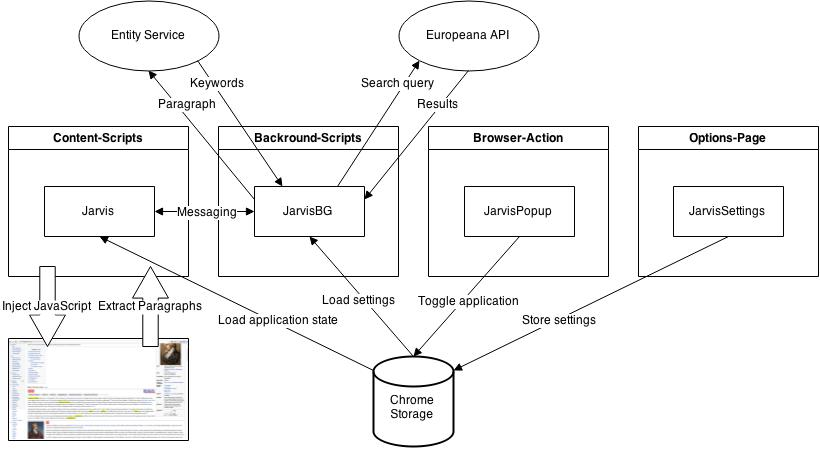
\includegraphics[width=\linewidth]{Bilder/architektur.jpg}
	\captionof{figure}{Kommunikation der AngularJS Komponenten untereinander}
	\label{fig:architektur}
 \end{minipage}
 
 Jarvis ist das Modul, welches in die jeweilige Webseite per JavaScript Injection eingefügt wird. Es extrahiert die Paragraphen aus dem Text und fügt die eigene Direktive in das DOM ein. Die extrahierten Paragraphen werden per Message Passing\footnote{\url{https://developer.chrome.com/extensions/messaging}} an die Background-Skripte weitergegeben. Diese sind zusammengefasst im Modul JarvisBG. 

 Dieses Modul ist zuständig für die Kommunikation mit den REST Endpunkten von Europeana und dem Keyword Service. Im Gegensatz zu Jarvis, welches für jeden offenen Browser-Tab eine eigene Instanz hat, existiert das JarvisBG Modul nur ein mal (wie auch JarvisPopup und JarvisSettings). Jarvis schickt Nachrichten mit dem Namen des angeforderten Services sowie einer Callback-Methode an JarvisBG. Dieses führt die Anfrage aus und übergibt die Ergebnisse der Callback-Methode. Diese sorgt dann dafür, dass die Ergebnisse im Frontend richtig angezeigt werden. 

 JarvisPopup ist das Modul des Popup-Fensters, welches nach klick auf das Icon der Extension rechts des Adressfeldes angezeigt wird. Über das Popup wird der Zustand der Extension im aktuellen Tab gesteuert. Der User kann hier entscheiden, ob das Programm in diesem Tab angezeigt wird oder nicht. Der Zustand wird dann im Chrome Storage\footnote{\url{https://developer.chrome.com/extensions/storage}} gespeichert. Die Wahl für die Speicherung der Anwendungsdaten viel auf den Chrome Storage, da er einige Vorteile gegenüber der localStorage API\footnote{\url{https://developer.mozilla.org/en-US/docs/Web/Guide/API/DOM/Storage\#localStorage}} bietet. Zum einen können die Content-Skripte direkt darauf zugreifen ohne einen Umweg über die Background-Skripte gehen zu müssen. Weiterhin erlaubt Chrome Storage eine automatische Synchronisierung der Inhalte. Dadurch wird Jarvis sofort benachrichtigt, sobald sich der Zustand der Applikation ändert.

 Der Nutzer hat die Möglichkeit, über die Options-Page\footnote{\url{https://developer.chrome.com/extensions/optionsV2}} die verwendeten Services zu konfigurieren. Das dafür zuständige Modul ist JarvisSettings. Es speichert die Einstellungen im Chrome Storage und JarvisBG passt die REST-Anfragen entsprechend an.

 \subsection{Paragraphen-Erkennung}
 
 \subsection{Paragraphen-Analyse}
 Um aus den gefundenen Paragraphen die wichtigen Schlüsselwörter zu extrahieren wird ein REST-Service genutzt, der vom Lehrstuhl für Medieninformatik an der Universität Passau bereitgestellt wurde. Dieser Service basiert auf DBpedia Spotlight\footnote{\url{http://spotlight.dbpedia.org/}}, einem System zur automatischen Annotation von DBpedia\footnote{\url{http://wiki.dbpedia.org/}} Entities in Texten \cite{daiber2013improving}. 

 DBpedia Spotlight ist ein Open Source Projekt welches einen REST-Service entwickelt hat, der Interfaces für Phrase Spotting (Erkennung von Ausdrücken die Annotiert werden können) und Disambiguierung (verlinken von Phrasen mit DBpedia Entities) anbietet. Es analysiert einen Text in vier Phasen. Während des Phrase Spottings
 
 the standart disambiguation algorithm is based upon cosine similarities and a modification of TD-IDF weights. main phrase spotting algorithm is exact string matching.
 the project has focused initially on the english language.

 phrase spotting: is the task of finding passages in a text that later should be linked to DBpedia entities. stardard phrase spotting algorithm used by DBpedia Spotlight is very light on its NLP demands, only requiring one language-dependent step: tokenization.
 candidates are generated:
 	1. identifying all sequences of capitalized tokens
 	2. identifying all noun phrases, prepositional phrases and multi word phrases
 	3. identifying all named entities

 german is available

 select the best candidates. all candidates below a score threshold are removed.
 score is computed for each spot candidate as a linear combination of features (annotation probability), binary features
 \cite{daiber2013improving}


 system for automatically annotating text documents with DBpedia URIs
 DBpedia spotlight computes scores such as prominence (how many times a resource is mentioned in wikipedia), topical relevance (how close a paragraph is to a DBpedia resource's context) and contextual ambiguity (is there more than one candidate resource with similarly high topical relevance for this surface form in its current context?)

 four stages: !spotting stage recognizes in a sentence the phrases that may indicate a mention of a DBpedia resource. 
 !candidate selection is subsequently employed to map the spotted phrase to resources that are candidate disambiguations for that phrase.
 the !disambiguation stage, in turn, uses the context around the spotted phrase to decide for the best choice amongst the candidates. 
 the annotation can be customized by users to their specific needs through !configuration parameters

 spotting:
 labels gathered from the DBpedia resources which can be seen as community approved surface forms.
 set of labels used used for spotting

 candidate selection:
 map resource names to candidate disambiguations. we use the dbpedia lexicalization dataset for determining candidate disambiguations for each surface form.
 the candidate selection offers a chance to narrow down the space of disambiguation possibilities
 candidate selection phase can also be viewed as a way to pre-rank the candidates for disambiguation before observing a surface form in the context of a paragraph

 disambiguation:
 after selecting candidate resources for each surface form, our system uses the context around the surface forms, e.g. paragraphs, as information to find the most likely disambiguations.
 we modeled dbpedia resource occurences in a Vector Space Model.
 our approach is to rank candidate resources according to the similarity score between their context vectors and the context surrounding the surface form.
 \cite{mendes2011dbpedia}

was kommt zurück: relevance score
nicht alle keywords werden angezeigt
 \subsection{Bau der GUIs}

\begin{minipage}{\linewidth}
	\centering
	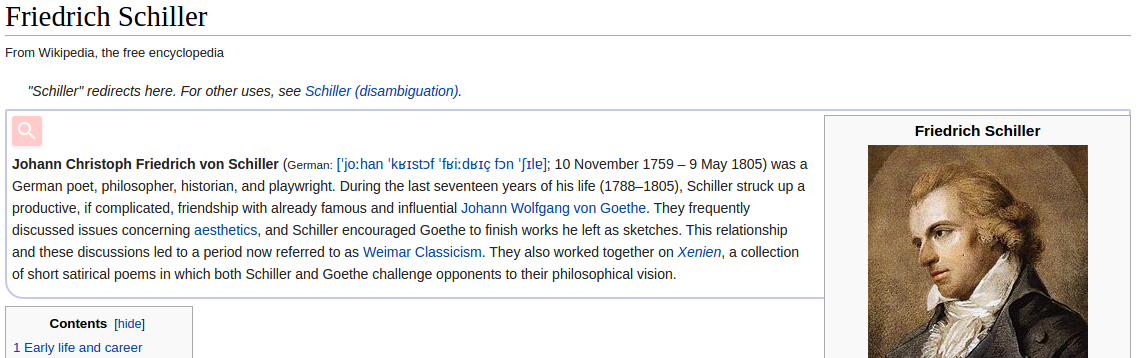
\includegraphics[width=\linewidth]{Bilder/app-screenshots/paragraph-unhovered.png}
	\captionof{figure}{Hervorgehobener Paragraph ohne Hover}
	\label{fig:paragraph}
 \end{minipage}
 \begin{minipage}{\linewidth}
	\centering
	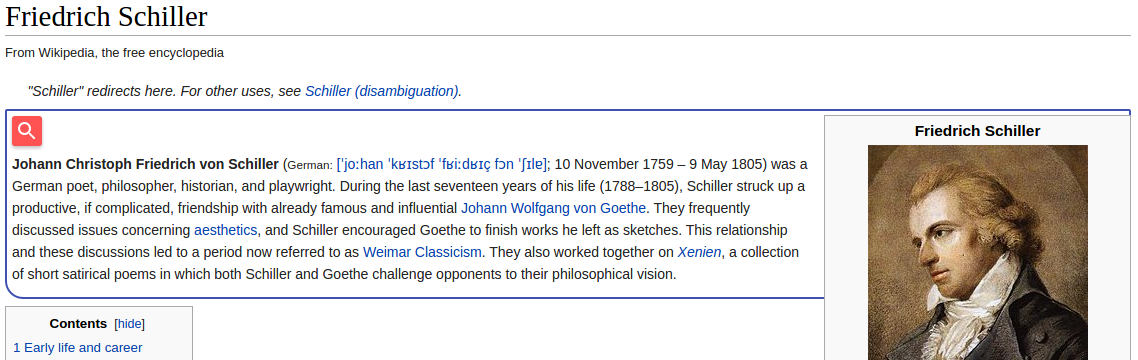
\includegraphics[width=\linewidth]{Bilder/app-screenshots/paragraph-hovered.png}
	\captionof{figure}{Hervorgehobener Paragraph mit Hover}
	\label{fig:paragraphHover}
 \end{minipage}
 \begin{minipage}{\linewidth}
	\centering
	\includegraphics[width=\linewidth]{Bilder/app-screenshots/keywords.png}
	\captionof{figure}{Anzeige der gefundenen Keywords sowie Anzahl der Ergebnisse}
	\label{fig:keywords}
 \end{minipage}
 \begin{minipage}{\linewidth}
	\centering
	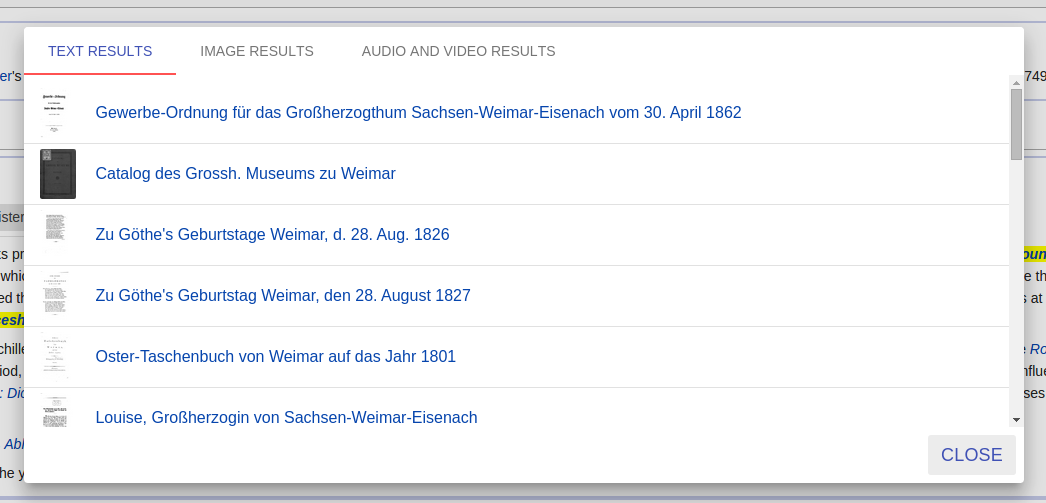
\includegraphics[width=\linewidth]{Bilder/app-screenshots/text-results.png}
	\captionof{figure}{Dialog mit gefundenen Textquellen}
	\label{fig:textResults}
 \end{minipage}
 \begin{minipage}{\linewidth}
	\centering
	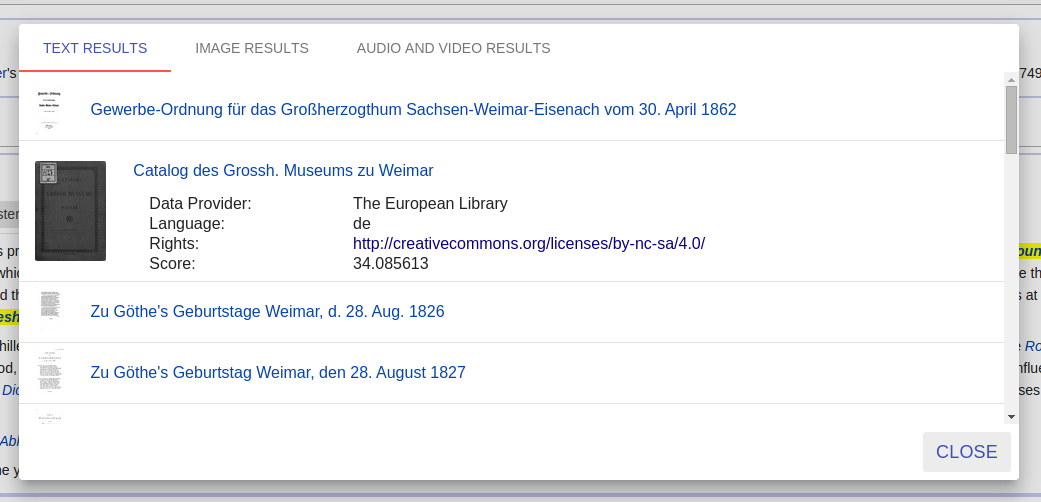
\includegraphics[width=\linewidth]{Bilder/app-screenshots/text-results-hovered.png}
	\captionof{figure}{Detaillierte Ansicht einer Textquelle}
	\label{fig:textResultsHover}
 \end{minipage}
 \begin{minipage}{\linewidth}
	\centering
	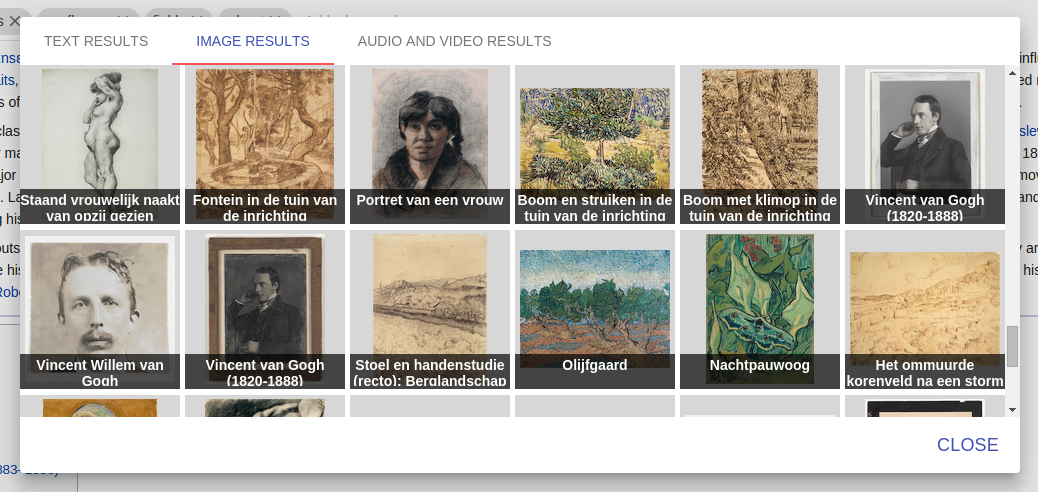
\includegraphics[width=\linewidth]{Bilder/app-screenshots/image-results.png}
	\captionof{figure}{Dialog mit gefundenen Bildquellen}
	\label{fig:imageResults}
 \end{minipage}
 \begin{minipage}{\linewidth}
	\centering
	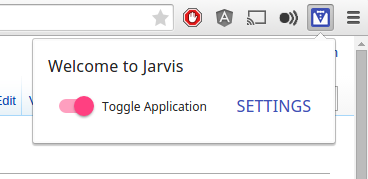
\includegraphics[scale=0.6]{Bilder/app-screenshots/popup.png}
	\captionof{figure}{Popup zum aktivieren der Extension}
	\label{fig:popup}
 \end{minipage}
 \begin{minipage}{\linewidth}
	\centering
	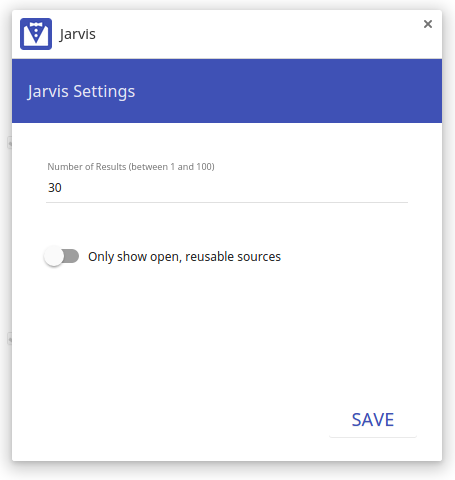
\includegraphics[scale=0.5]{Bilder/app-screenshots/settings.png}
	\captionof{figure}{Dialog zum anpassen der Einstellungen}
	\label{fig:settings}
 \end{minipage}

		- > Darf den Benutzer nicht zu sehr ablenken
		- > Ergebnisse müssen in der Nähe ihrer „Quelle“ angezeigt werden (proximity compatibility pricinple)
		- > Benutzer muss klar zwischen Webseite und Augmentation unterscheiden können
		- > buntes, auffälliges Design
		- > Ramping interface: Mehr Benutzerinteraktionen führen zu mehr angezeigten Informationen (Erklärung der Stages) 


 Durch die Chips kann man später auch leicht IQE hinzufügen, zb relevance feedback

 Probleme mit Hyperlinks
 \subsection{Einbindung der REST-Services}